\chapter{Theoretische Grundlagen}
\label{chap:theoretische_grundlagen} Dieses Kapitel führt in die theoretischen Grundlagen
ein, die in dieser Arbeit benötigt werden. Den ersten Teil bilden die domänenspezifischen
Grundlagen \ref{sec:domänenspezifisch}, welche genauer darauf eingehen, welchen Inhalt
die zu bearbeitenden Bilder bieten und wie dieser zu verstehen ist. Abschnitt
\ref{sec:technologisch} geht hierbei auf verschiedenen Technologien ein, die eine
wichtige Rolle spielen. Der Abschnitt \ref{sec:verwwandte_arbeit} geht auf die
Arbeit vin \citet{hoffmann2020} ein und legte damit den Grundstein diese vorliegenden
Arbeit. Die Abschnitte \ref{sec:3d_slicer} und \ref{sec:architektonisch} führen
in Softwareentwicklungsthemen ein, die zum erstellen einer \textit{3D Slicer
Extention} wichtig sind.

\section{Domänenspezifisch}
\label{sec:domänenspezifisch} Wie bereits aus dem Kapitel \ref{chap:einleitung}
Einleitung klar wurde, handelt es sich bei den Micro-CT Bilder um Zahnbilder,
die aufgrund einer Karieserkrankung entfernt wurden. Um zu verstehen, wie eine
CT-Aufnahme eines Zahns augeteilt werden soll, ist es hilfreich zu verstehen,
wie ein Zahn aufgebaut ist.

\begin{minipage}{0.40\textwidth}
	Die Abbildung \ref{fig:aufbau_eines_zahnes} zeigt den groben Aufbau eines Zahnes
	nach \citet[Seite 17]{lehmann2012Zahnheilkunde}. Zu sehen ist, dass das Denit oder
	auch Zahnbein genannt, den Großteil eines Zahnes einnimmt. Im bereich der Zahnkrone
	wird das Dentin von Zahnschmelz überzogen. Der Zahnschmelz ragt in die
	Mundhöle und ist nach \cite[Seite 41]{lehmann2012Zahnheilkunde} das härteste
	Material im menschlichen Körper. In der Mitte des Zahnes befindet sich Weichgewebe,
	welches als Pulpa bezeichnet wird vgl. \citep[Seite ]{lehmann2012Zahnheilkunde}.
\end{minipage}
\hfill
\begin{minipage}{0.50\textwidth}
	\centering
	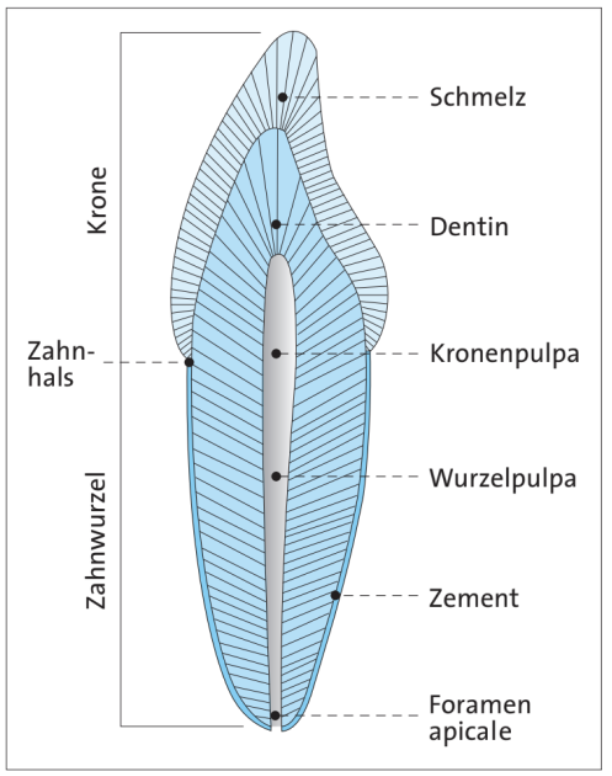
\includegraphics[scale=0.50]{img/aufbau_eines_zahns.jpg}
	\captionof{figure}{Aufbau eines Zahnes nach \citet{lehmann2012Zahnheilkunde}} \label{fig:aufbau_eines_zahnes}
\end{minipage}

Für die Bearbeitung von Micro-CT Aufnahmen sind die Bereich Schmelz Dentin und Pulpa
von besonderer Bedeutung. Betrachtet man eine CT wie es zu begin in der
Abbildung \ref{fig:ct_aufnahme_eines_zahns} gezeigt wurde, so bilden diese 3 Gewebearten
die unterschiedlichen Grauwerte in einem CT-Bild. Die \textbf{Pulpa} unterscheidet sich
hierbei nur wenig vom Hintergrund, da sie als einzige der drei Hauptteile eines Zahnes
eine Weichgewebe ist und bei einer Röntgenaufnahme nicht absorbiert. Geht man weiter von innen nach außen, so ist der nächste Zahnteil auf einem CT das Zahnbein. Das
\textbf{Dentin} ist laut \citet[Seite 41]{lehmann2012Zahnheilkunde} eine Hartsubstanz, die dem Kieferknochen sehr nahe steht. So kommt es, dass dieser Teil schon deutlich besser auf einem CT zu erkennen ist. Den äußersten Teil in der Mundhöle bildet der
\textbf{Schmelz}. Wie bereits erwähnt ist er der härteste Teil im menschlichen Körper und
aus diesem Grund auch am hellsten auf dem CT zu erkennen. Die beiden folgenden Abbildungen sollen durch gegenüberstellung den Zusammenhang zwischen einem CT-Bild und einer Zahnzeichnung verdeutlichen.

\begin{minipage}{0.45\textwidth}
    \centering
	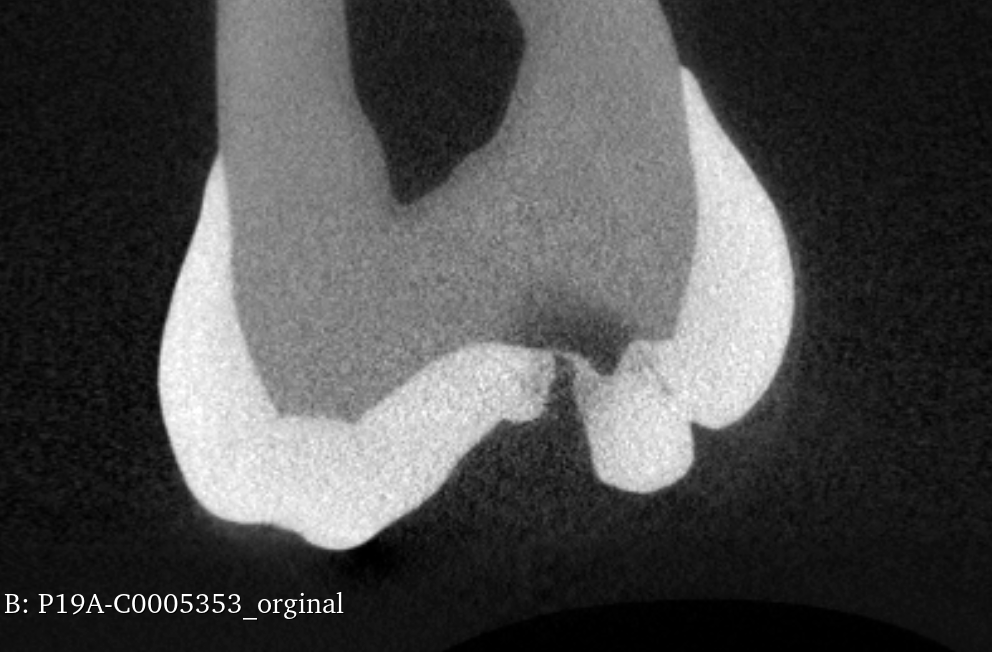
\includegraphics[scale=0.2]{img/vgl_ct_zeichnung_ct.jpg}
    \label{fig:aufbau_eines_zahnes}
\end{minipage}
\hfill
\begin{minipage}{0.45\textwidth}
	\raggedleft
	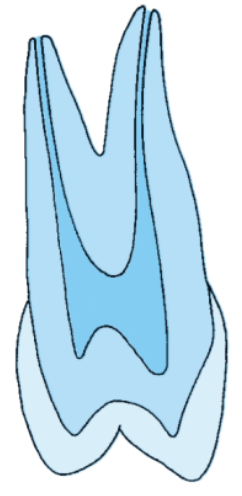
\includegraphics[scale=0.65]{img/vgl_ct_zeichnung_zeichnung.jpg}
    \label{fig:aufbau_eines_zahnes}
\end{minipage}



\section{Technologisch}
\label{sec:technologisch}

\section{Verwandte Arbeit}
\label{sec:verwwandte_arbeit}

\section{3D Slicer}
\label{sec:3d_slicer}

\section{Architektonisch}
\label{sec:architektonisch}